\section{Графический вывод}
\label{sec:graphical_display}

При графическом выводе следующие элементы являются базовыми: начальная точка
(reference point), графический контекст, цвет, изображение, закраска замкнутых
фигур, тексты и растровые изображения.

\subsection{Ориентир и графический контекст}
\label{subsec:reference_point_and_graphical_context}

Библиотека \code{Graphics} управляет единственным и главным окном. Координаты
ориентира окна могут меняться от нижней левой точки (0,0) до верхнего правого
угла. Вот основные операции над этим окном:

\begin{itemize}
	\item \code{open\_graph}, типа \type{string -> unit}, которая открывает 
окно

	\item \code{close\_graph}, типа \type{unit -> unit}, которая закрывает 
его

	\item \code{clear\_graph}, типа \type{unit -> unit}, которая очищает его
\end{itemize}

Размер окна определяется функциями \code{size\_x} и \code{size\_y}.

Строка, которую мы передаём функции \code{open\_graph}, зависит от графической
оболочки машины где запускается программа, то есть она платформо зависимая. Если
строка пустая, то полученное окно будет иметь свойства по умолчанию. Мы можем
явно указать размер окна; в X-Window строка \code{`` $200 \times 300$''} 
создаст окно размером 200 пискелей по ширине и 300 по высоте. Заметьте, пробел 
--- первый символ строки \code{`` $200 \times 300$''} обязателен.

В графическом контексте есть несколько параметров которые можно 
просмотреть и изменить:

\begin{tabular}{rl}
	текущая точка: & \type{current\_point : unit -> int * int} \\
	 &  \code{moveto} : \type{int -> int -> unit} \\
	текущий цвет : & \type{set\_color : color -> unit} \\
	ширина текущей линии : & \type{set\_line\_width : int -> unit} \\
	текущий шрифт : & \type{set\_font : string -> unit} \\
	размер этого шрифта : & \type{set\_text\_size : int -> unit} \\
\end{tabular}

\subsection{Цвета}
\label{subsec:colors}

Цвет представлен тремя байтами, каждый из которых хранит яркость основного
цвета в модели RGB (red, green, blue) в интервале от 0 до 255. Функция 
\code{rgb} (с типом \type{int -> int -> int -> color}) создаёт цвет с тремя 
указанными значениями. Если все три значения равны, то мы получим серый цвет 
более или менее светлый, в зависимости от значений. Чёрный соответствует 
минимуму яркости для каждой компоненты цвета \code{(0,0,0)}, белый цвет --- 
\code{(255,255,255)}. Есть некоторые предопределённые цвета: \code{black, 
white, red, green, blue, yellow, cyan, magenta}.

Переменные \code{foreground} и \code{background} соответствуют текущему 
цвету и цвету фона. При стирании экрана, осуществляется заполнение цветом фона.

Цвет (значение типа \type{color}) это на самом деле целое число, которое мы
можем разбить на три части (\code{from\_rgb}) или инвертировать
(\code{inv\_color}).

\begin{lstlisting}[language=OCaml]
(* color == R * 256 * 256  +  G * 256  +  B  *)
# let from_rgb (c : Graphics.color)  =
   let r = c / 65536  and  g = c / 256 mod 256  and  b = c mod 256
   in (r,g,b);;
val from_rgb : Graphics.color -> int * int * int = <fun>
# let inv_color (c : Graphics.color) =
    let (r,g,b) = from_rgb c
    in Graphics.rgb (255-r) (255-g) (255-b);;
val inv_color : Graphics.color -> Graphics.color = <fun>
\end{lstlisting}

Функция \code{point\_color}, типа \type{int -> int -> color}, возвращает
цвет точки, координаты которой указаны на входе.

\subsection{Рисунок и заливка}
\label{subsec:drawing_and_filling}

Функция рисования выводит линию на экран, при этом для толщины и цвета
используются текущие значения. Функция заливки закрашивает замкнутую форму
текущим цветом. Различные функции рисования и заливки приведены в таблице
\ref{tbl:drawing_and_filling_functions}

Функции рисования и заливки
\begin{table}[hl]
	\begin{center}
	\caption{\label{tbl:drawing_and_filling_functions} Функции рисования и
заливки}
	\begin{tabular}{|l|l|r|}
		\hline
		рисунок & заполнение & тип \\
		\hline
		\code{plot} & & \type{int -> int -> unit} \\
		\hline
		\code{lineto} & & \type{int -> int -> unit} \\
		\hline
		& \code{fill\_rect} & \type{int -> int -> int -> int -> unit} \\
		\hline
		& \code{fill\_poly} & \type{( int * int) array -> unit} \\
		\hline
		\code{draw\_arc} & \code{fill\_arc} & \type{int -> int -> int -> int -> 
int -> unit} \\
		\hline
		\code{draw\_ellipse} & \code{fill\_ellipse} & \type{int -> int -> int 
-> int -> unit} \\
		\hline
		\code{draw\_circle} & \code{fill\_circle} & \type{int -> int -> int -> 
unit} \\
		\hline
	\end{tabular}
	\end{center}
\end{table}

Заметьте, что функция \code{lineto} имеет побочный эффект: она изменяет
положение текущей точки.

\subsubsection{Рисование многоугольников}

В следующем примере, мы добавим некоторые функции рисования, которые не 
существуют в библиотеке. Многоугольник определяется вектором его вершин.

\begin{lstlisting}[language=OCaml]
# let draw_rect x0 y0 w h = 
   let (a,b) = Graphics.current_point() 
   and x1 = x0+w and y1 = y0+h 
   in
     Graphics.moveto x0 y0; 
     Graphics.lineto x0 y1; Graphics.lineto x1 y1;  
     Graphics.lineto x1 y0; Graphics.lineto x0 y0; 
     Graphics.moveto a b  ;;
val draw_rect : int -> int -> int -> int -> unit = <fun>

# let draw_poly r =
   let (a,b) = Graphics.current_point () in 
   let (x0,y0) = r.(0) in Graphics.moveto x0 y0 ; 
     for i = 1 to (Array.length r)-1 do
       let (x,y) = r.(i) in Graphics.lineto x y
     done ;
     Graphics.lineto x0 y0 ;
     Graphics.moveto a b ;;
val draw_poly : (int * int) array -> unit = <fun>
\end{lstlisting}

Обратите внимание на то что эти функции берут такие же аргументы что и 
существующие функции заливки. Так они не изменяют состояние текущей точки.

\subsubsection{Модель художника}

Следующий пример иллюстрирует сеть эстафетного кольца (token ring) 
(\ref{fig:token_ring_network}). Каждый компьютер представлен в виде небольшого 
круга, все компьютеры соединены между собой и сеть образует кольцо. Текущее 
положение маркера в сети изображено чёрным кругом.

Функция \code{net\_points} создаёт координаты всех компьютеров сети, эти данные 
будут храниться в векторе.

\begin{lstlisting}[language=OCaml]
# let pi = 3.1415927 ;;
val pi : float = 3.1415927
# let ens_points (x,y) l n = 
   let a = 2. *. pi /. (float n) in
   let rec aux (xa,ya) i = 
     if i > n then [] 
     else 
       let na = (float i) *. a in 
       let x1 = xa + (int_of_float ( cos(na) *. l))
       and y1 = ya + (int_of_float ( sin(na) *. l))  in
       let np = (x1,y1) in
         np::(aux np (i+1)) 
   in Array.of_list (aux (x,y) 1) ;;
val ens_points : int * int -> float -> int -> (int * int) array = <fun>
\end{lstlisting}

Функция \code{draw\_net} выводит соединения, компьютеры и маркер.

\begin{lstlisting}[language=OCaml]
# let dessine (x,y) l n sc st = 
  let r = ens_points (x,y) l n in 
    draw_poly r ;
    let dessine_cercle (x,y) = 
      Graphics.set_color Graphics.background ; 
      Graphics.fill_circle x y sc ; 
      Graphics.set_color Graphics.foreground ; 
      Graphics.draw_circle x y sc
    in 
      Array.iter dessine_cercle r ;
      Graphics.fill_circle x y st ;;
val dessine : int * int -> float -> int -> int -> int -> unit = <fun>
\end{lstlisting}

При следующем вызове получим левую картинку на рисунке 
\ref{fig:token_ring_network}.

\begin{lstlisting}[language=OCaml]
# dessine (140,20) 60.0 10 10 3;;
- : unit = ()
\end{lstlisting}

\begin{lstlisting}[language=OCaml]
# save_screen "IMAGES/tokenring.caa";;
- : unit = ()
\end{lstlisting}

\begin{figure}[h]
	\center{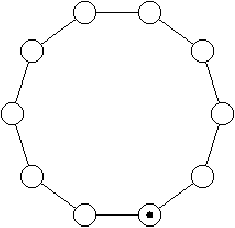
\includegraphics[scale=0.5]{drafts/book-ora007}
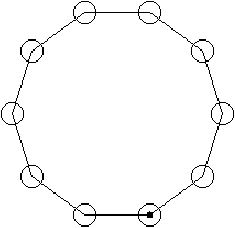
\includegraphics[scale=0.5]{drafts/book-ora008}}
	\caption{\label{fig:token_ring_network}Сеть эстафетное кольцо}
\end{figure}

\subsection{Текст}
\label{subsec:text}

Две следующие функции вывода текста на экран чрезвычайно просты: 
\code{draw\_char} (с типом \type{char -> unit}) и \code{draw\_string} (с типом 
\type{string -> unit}) выводят на экран один символ и строку соответственно. 
Вывод осуществляется на текущую позицию экрана, также эти обе функции учитывают 
значение текущего шрифта и его размер.

{\it Замечание}

Вывод текста на экран может зависеть от графической оболочки.
Для переданной в аргументе строки, функция \code{text\_size} возвращает пару 
целых чисел, которые соответствуют размерам выведенной строки с текущим шрифтом 
и размером.

\subsubsection{Вертикальный вывод текста}

В следующем примере функция \code{draw\_string\_v} вертикально выводит на экран 
строку начиная с текущей позиции. Результат изображён на рисунке 
\ref{fig:legend_around_axes}, каждая буква выводится отдельно, меняя 
вертикальные координаты.

\begin{lstlisting}[language=OCaml]
# let draw_string_v  s = 
   let (xi,yi) = Graphics.current_point() 
   and l = String.length s 
   and (_,h) = Graphics.text_size s 
   in 
      Graphics.draw_char s.[0] ;
      for i=1 to l-1 do
        let (_,b) = Graphics.current_point() 
        in Graphics.moveto xi (b-h) ;
           Graphics.draw_char s.[i] 
       done ;
     let (a,_) = Graphics.current_point() in Graphics.moveto a yi ;;
val draw_string_v : string -> unit = <fun>
\end{lstlisting}

Эта функция изменяет текущую позицию, после вывода позиция перемещается на 
расстояние равное ширине символа.

Следующая программа выводит легенду вдоль координатных осей (рис. 
\ref{fig:legend_around_axes}).

\begin{lstlisting}[language=OCaml]
#
 Graphics.moveto 0 150   ; Graphics.lineto 300 150 ;
 Graphics.moveto 2 130   ; Graphics.draw_string "abscisses" ;
 Graphics.moveto 150 0   ; Graphics.lineto 150 300 ;
 Graphics.moveto 135 280 ; draw_string_v "ordonnées" ;;
- : unit = ()
\end{lstlisting}

\begin{figure}[h]
	\center{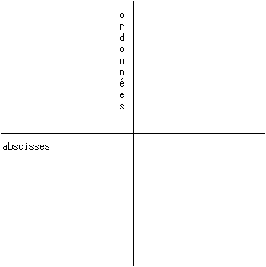
\includegraphics[scale=0.5]{drafts/book-ora009}}
	\caption{\label{fig:legend_around_axes}Легенда координатных осей}
\end{figure}

Для того чтобы вывести вертикальный текст, необходимо помнить что функция 
\code{draw\_string\_v} изменяет текущую позицию. Для этого определим функцию 
\code{draw\_text\_v} с двумя аргументами: расстояние между столбцами и список 
слов.

\begin{lstlisting}[language=OCaml]
# let draw_text_v n l = 
   let f s = let (a,b) = Graphics.current_point() 
             in draw_string_v s ;
                Graphics.moveto (a+n) b
   in List.iter f l ;;
val draw_text_v : int -> string list -> unit = <fun>
\end{lstlisting}

Если необходимо реализовать другие манипуляции с текстом, такие, как вращение, 
мы должны использовать растр каждой буквы и произвести вращение всех пикселей.

\subsection{Растровые изображения}
\label{subsec:bitmaps}

Растровое изображение может быть представлено либо как матрица цветов 
\type{(color array array)}, либо как значение абстрактного типа 
\footnote{абстрактным называется тип представление которого не известно. 
Объявление подобных типов рассматривается в главе \ref{??}} \type{image} из 
библиотеки \code{Graphics}. Имена и типы функций приведены в таблице 
\ref{tbl:functions_for_manipulating_bitmaps}.

\begin{table}[hl]
	\begin{center}
	\caption{\label{tbl:functions_for_manipulating_bitmaps} Функции работы с 
растром}
	\begin{tabular}{|l|l|}
		\hline
		функция & тип \\
		\hline
		\code{make\_image} & \type{color array array -> image} \\
		\hline
		\code{dump\_image} & \type{image -> color array array} \\
		\hline
		\code{draw\_image} & \type{image -> int -> int -> unit} \\
		\hline
		\code{get\_image} & \type{int -> int -> int -> int -> image} \\
		\hline
		 \code{blit\_image} & \type{image -> int -> int -> unit} \\
		\hline
		 \code{create\_image} & \type{int -> int -> image} \\
		\hline
	\end{tabular}
	\end{center}
\end{table}

Функции \code{make\_image} и \code{dump\_image} конвертируют из одного типа в 
другой --- \type{image} и \type{color array array}. Функция \code{draw\_image} 
выводит на экран растр начиная с координат его нижнего левого угла.

При помощи функции \code{get\_image} мы можем захватить прямоугольную часть 
экрана и создать таким образом изображение, для этого необходимо указать нижнюю 
левую и правую верхнюю углы зоны захвата. Функция \code{blit\_image} 
захватывает экран часть экрана и сохраняет изображение которое мы передали в 
виде аргумента (тип \type{image}), второй аргумент указывает нижний левый угол 
части экрана, которую мы желаем захватить. Размер захватываемой части зависит 
от размеров изображения, переданного в аргументе. Функция \code{create\_image} 
инициализирует изображение, для этого необходимо указать его будущий размер. 
Позднее, это изображение мы можем изменить функцией \code{blit\_image}.

Предопределённый цвет \code{transp} позволяет сделать точки изображения 
прозрачными. Это позволяет нам вывести изображение лишь на части прямоугольника, 
прозрачные точки не изменяют начальный экран.

\subsubsection{Поляризация Jussieu}\footnote{Jussieu --- здание парижского 
университета. Там в частности находится известная Лаборатория Информатики 
Париж-6 (lip6), где работают авторы книги, прим. пер.}

В следующем примере мы инвертируем цвет точек растра, для чего будем 
использовать функцию, которая была представлена в \ref{subsec:colors}, для 
каждого пикселя растра.

\begin{lstlisting}[language=OCaml]
# let inv_image i = 
   let inv_vec = Array.map (fun c -> inv_color c) in
   let inv_mat = Array.map inv_vec  in 
   let matrice_inversee = inv_mat (Graphics.dump_image i) in 
   Graphics.make_image matrice_inversee ;;
val inv_image : Graphics.image -> Graphics.image = <fun>
\end{lstlisting}

На рисунке \ref{fig:inversion_of_Jussieu}, картинка слева --- начальное 
изображение и правое --- новое, \enq{освещённое солнцем}, после использование 
функции \code{inv\_image}.

\begin{lstlisting}[language=OCaml]
# let f_jussieu2 () = inv_image jussieu1;; 
val f_jussieu2 : unit -> Graphics.image = <fun>
\end{lstlisting}

\begin{figure}[h]
	\center{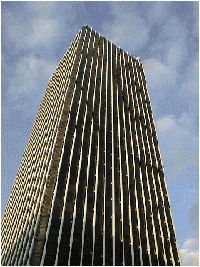
\includegraphics[scale=0.7]{drafts/book-ora010}
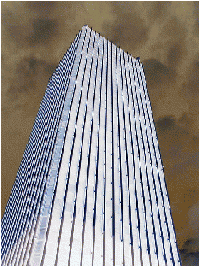
\includegraphics[scale=0.7]{drafts/book-ora011}}
	\caption{\label{fig:inversion_of_Jussieu}Инверсия Jussieu}
\end{figure}

\subsection{Пример: рисование рельефных блоков}
\label{subsec:example_drawing_of_boxes_with_relief_patterns}

В этом примере мы попытаемся определить несколько полезных функций вывода 
рельефных блоков. Блоком мы называем общий объект, который послужит в 
дальнейшем. Блок вписывается в прямоугольник, который задан начальной точкой, 
высотой и шириной.

Для того чтобы придать блоку рельефный вид, достаточно добавить две трапеции 
светлых тонов и две более тёмных.

\begin{figure}[h]
	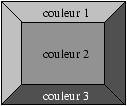
\includegraphics[scale=0.4]{drafts/book-ora012}
\end{figure}

Инвертируя цвета можно создать впечатление вогнутого или выпуклого блока.

\begin{figure}[h]
	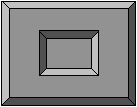
\includegraphics[scale=0.4]{drafts/book-ora013}
\end{figure}

\subsubsection{Реализация}

Добавим новые свойства блока: толщина окантовки, тип вывода на экран (выпуклый, 
вогнутый или плоский), цвета окантовки и фона. Вся эта информация сгруппирована 
в записи.

\begin{lstlisting}[language=OCaml]
# type relief = Top | Bot | Flat ;;
# type box_config =
  { x:int; y:int; w:int; h:int; bw:int; mutable r:relief ;
    b1_col : Graphics.color ;
    b2_col : Graphics.color ;
    b_col : Graphics.color} ;;
\end{lstlisting}

Только поле \code{r} может быть изменено. Для вывода на экран мы используем 
функцию рисующую прямоугольник \code{draw\_rect}, которую мы определили на 
\ref{subsec:drawing_and_filling}.

Для удобства, определим функцию рисующую контур блока.

\begin{lstlisting}[language=OCaml]
# let draw_box_outline bcf col = 
  Graphics.set_color col ;
  draw_rect bcf.x bcf.y bcf.w  bcf.h ;;
val draw_box_outline : box_config -> Graphics.color -> unit = <fun>
\end{lstlisting}

Функция вывода на экран состоит из трёх частей: рисование первой окантовки, 
затем второй и внутренней части блока.

\begin{lstlisting}[language=OCaml]
# let draw_box bcf = 
   let x1 = bcf.x and y1 = bcf.y in
   let x2 = x1+bcf.w and y2 = y1+bcf.h in 
   let ix1 = x1+bcf.bw and ix2 = x2-bcf.bw 
   and iy1 = y1+bcf.bw and iy2 = y2-bcf.bw in 
   let border1 g =
     Graphics.set_color g;
     Graphics.fill_poly 
       [| (x1,y1);(ix1,iy1);(ix2,iy1);(ix2,iy2);(x2,y2);(x2,y1) |] 
   in
   let border2 g = 
     Graphics.set_color g;
     Graphics.fill_poly 
       [| (x1,y1);(ix1,iy1);(ix1,iy2);(ix2,iy2);(x2,y2);(x1,y2) |]
   in
   Graphics.set_color bcf.b_col;
   ( match bcf.r with
         Top  -> 
           Graphics.fill_rect ix1 iy1 (ix2-ix1) (iy2-iy1) ;
           border1 bcf.b1_col ; 
           border2 bcf.b2_col
       | Bot  -> 
           Graphics.fill_rect ix1 iy1 (ix2-ix1) (iy2-iy1) ;
           border1 bcf.b2_col ; 
           border2 bcf.b1_col
       | Flat -> 
           Graphics.fill_rect x1 y1 bcf.w bcf.h ) ;
   draw_box_outline bcf Graphics.black ;;
val draw_box : box_config -> unit = <fun>
\end{lstlisting}

Контур блока подсвечен чёрным цветом. Для того чтобы стереть блок, достаточно 
заполнить пространство фоновым цветом.

\begin{lstlisting}[language=OCaml]
# let erase_box bcf = 
    Graphics.set_color bcf.b_col ; 
    Graphics.fill_rect (bcf.x+bcf.bw) (bcf.y+bcf.bw) 
                       (bcf.w-(2*bcf.bw)) (bcf.h-(2*bcf.bw)) ;;
val erase_box : box_config -> unit = <fun>
\end{lstlisting}

И наконец, определим функцию выводящую текст выровненный слева, справа или по 
центру блока. Для описания позиции текста в блоке определим тип \type{position}.

\begin{lstlisting}[language=OCaml]
# type position = Left | Center | Right ;; 
type position = | Left | Center | Right
# let draw_string_in_box pos str bcf col = 
     let (w, h) = Graphics.text_size str in
     let ty = bcf.y + (bcf.h-h)/2 in 
     ( match pos with 
           Center -> Graphics.moveto (bcf.x + (bcf.w-w)/2) ty 
         | Right  -> let tx = bcf.x + bcf.w - w - bcf.bw - 1 in 
                     Graphics.moveto tx ty 
         | Left   -> let tx = bcf.x + bcf.bw + 1 in Graphics.moveto tx ty  ) ;
     Graphics.set_color col ;
     Graphics.draw_string str ;;
val draw_string_in_box :
  position -> string -> box_config -> Graphics.color -> unit = <fun>
\end{lstlisting}

\subsubsection{Пример: рисование игры}

Чтобы продемонстрировать использование блоков, выведем на экран поле игры 
\enq{крестики--нолики}, как на рисунке \ref{fig:displaying_of_boxes_with_text}. 
Для упрощения задачи, определим цвета для игры.

\begin{lstlisting}[language=OCaml]
# let set_grey x =  (Graphics.rgb x x x) ;;
val set_grey : int -> Graphics.color = <fun>
# let grey1= set_grey 100 and grey2= set_grey 170 and grey3= set_grey 240 ;;
val grey1 : Graphics.color = 6579300
val grey2 : Graphics.color = 11184810
val grey3 : Graphics.color = 15790320
\end{lstlisting}

Теперь, напишем функцию рисующую матрицу блоков одного размера. 

\begin{lstlisting}[language=OCaml]
# let rec create_grid nb_col n sep b  =
   if n < 0 then []
   else 
     let px = n mod nb_col and py = n / nb_col in
     let nx = b.x +sep + px*(b.w+sep)
     and ny = b.y +sep + py*(b.h+sep) in
     let b1 = {b with x=nx; y=ny} in
     b1::(create_grid nb_col (n-1) sep b) ;;
val create_grid : int -> int -> int -> box_config -> box_config list = <fun>
\end{lstlisting}

Создадим список блоков. 

\begin{lstlisting}[language=OCaml]
# let vb = 
   let b =  {x=0; y=0; w=20;h=20; bw=2;
             b1_col=grey1; b2_col=grey3; b_col=grey2; r=Top} in 
   Array.of_list (create_grid 5 24 2  b) ;;
val vb : box_config array =
  [|{x=90; y=90; w=20; h=20; bw=2; r=Top; b1_col=6579300; b2_col=15790320;
     b_col=11184810};
    {x=68; y=90; w=20; h=20; bw=2; r=Top; b1_col=6579300; b2_col=15790320;
     b_col=...};
    ...|]
\end{lstlisting}

Изображение \ref{fig:displaying_of_boxes_with_text} соответствует результату 
следующих вызовов:

\begin{lstlisting}[language=OCaml]
# Array.iter draw_box vb ;
 draw_string_in_box Center "X" vb.(5) Graphics.black ;
 draw_string_in_box Center "X" vb.(8) Graphics.black ;
 draw_string_in_box Center "O" vb.(12) Graphics.yellow ;
 draw_string_in_box Center "O" vb.(11) Graphics.yellow ;;
- : unit = ()
\end{lstlisting}

\begin{figure}[h]
	\center{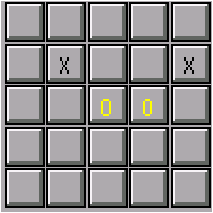
\includegraphics[scale=0.5]{drafts/book-ora014}}
	\caption{\label{fig:displaying_of_boxes_with_text}Вывод блоков с текстом}
\end{figure}
